

\chapter{Complex Number and Low Pass Simulation}

\underline{References:} chapter 5 in \cite{book_SDR_BobStewart} and chapter 4 in \cite{book_comm_system_sim_Tranter}

\section{Review of Basics}

\begin{itemize}

\item Advantage of complex notation: easier to work with multiplication of complex exponential rather then the multiplication of 2 cos

    \begin{itemize}
        \item $e^{j \, A} \, e^{j \, B} \, = \, e^{j \, (\, A \, + \, B \, )}$
        
        \item $\cos(A) \, \cos(B) \, = \, \displaystyle\frac{1}{2} \, \left[\, \cos( \, A \, + \, B \, ) \, + \, \cos( \, A \, - \, B \, )    \, \right]$
    \end{itemize}

\item Signal processing work with voltages to process real world quantities

\begin{itemize}
    \item When the antenna see the change in the EM field, it induces voltages
    
    \item Microphone pick up sound waves from small changes in sound pressure to produce voltage
\end{itemize}


\end{itemize}


\newpage
\section{Quadrature Representation}


\subsection{Case Usage}

IQ signals are used in many places. In communication applications:

\begin{itemize}
    \item Used in Tx side to \tbi{unify many modulation scheme} (as shown in \autoref{fig:Sampling:qudrature_impelmentation})
    
    \begin{itemize}
        \item Instead of using different circuitry for each modulation type, we can change the IQ values to obtain various modulation type
    \end{itemize}
    

\item Used in Rx for demodulation as shown in \autoref{fig:Sampling:I_Q_system}

\begin{figure}[h]
\centering
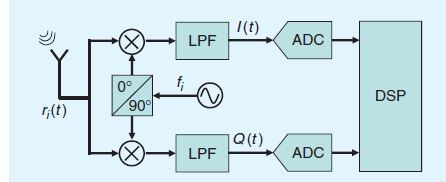
\includegraphics[width = 0.7\textwidth]{Figures/Sampling/I_Q_system}
\caption{A block diagram of a typical I-Q demodulator \cite{Sub_Nyquist_sampling}}
\label{fig:Sampling:I_Q_system}
\end{figure}


    
\end{itemize}

\todo{Case Usage}

\textit{Try to simulate these idea in practical application}



\subsection{Formula}


\begin{equation}
\begin{array}{lll}
x_{\text{band-pass}}(t) \, &=&\, \text{Amp}(t) \, \times \, \text{cos}\left(\, 2 \pi \, f_{\text{center}} \, t \, + \, \text{phase}(t) \,\right)\\ \\
        &=& \, x_{\text{in-phase}}(t) \, \text{cos}\left(\, 2 \pi \, f_{\text{center}} \, t \,\right) + \, x_{\text{quadrature}}(t) \, \text{sin}\left(\, 2 \pi \, f_{\text{center}} \, t \,\right) 
\end{array}
\label{Eq:Sampling:based_band_general_form_time_domain}
\end{equation}

where $\begin{cases}
x_{\text{Eq-Baseband}}(t) \, = \, \text{Amp}(t)\,\times \, \text{exp}\left[\, j \,\times \, \text{phase}(t) \,\right] \\ \\
\text{Amp}(t) \, = \, \sqrt{ x_{\text{in-phase}}^2(t) \, + \, x_{\text{quadrature}}^2(t)} \\ \\
\text{phase}(t) \,  = \, \text{tan}^{-1}\left[\, \displaystyle\frac{ x_{\text{quadrature}}(t)}{x_{\text{in-phase}}(t)} \,\right] 
\end{cases}$



\newpage

\subsection{Summary for IQ Representation}

\begin{figure}[h]
\centering
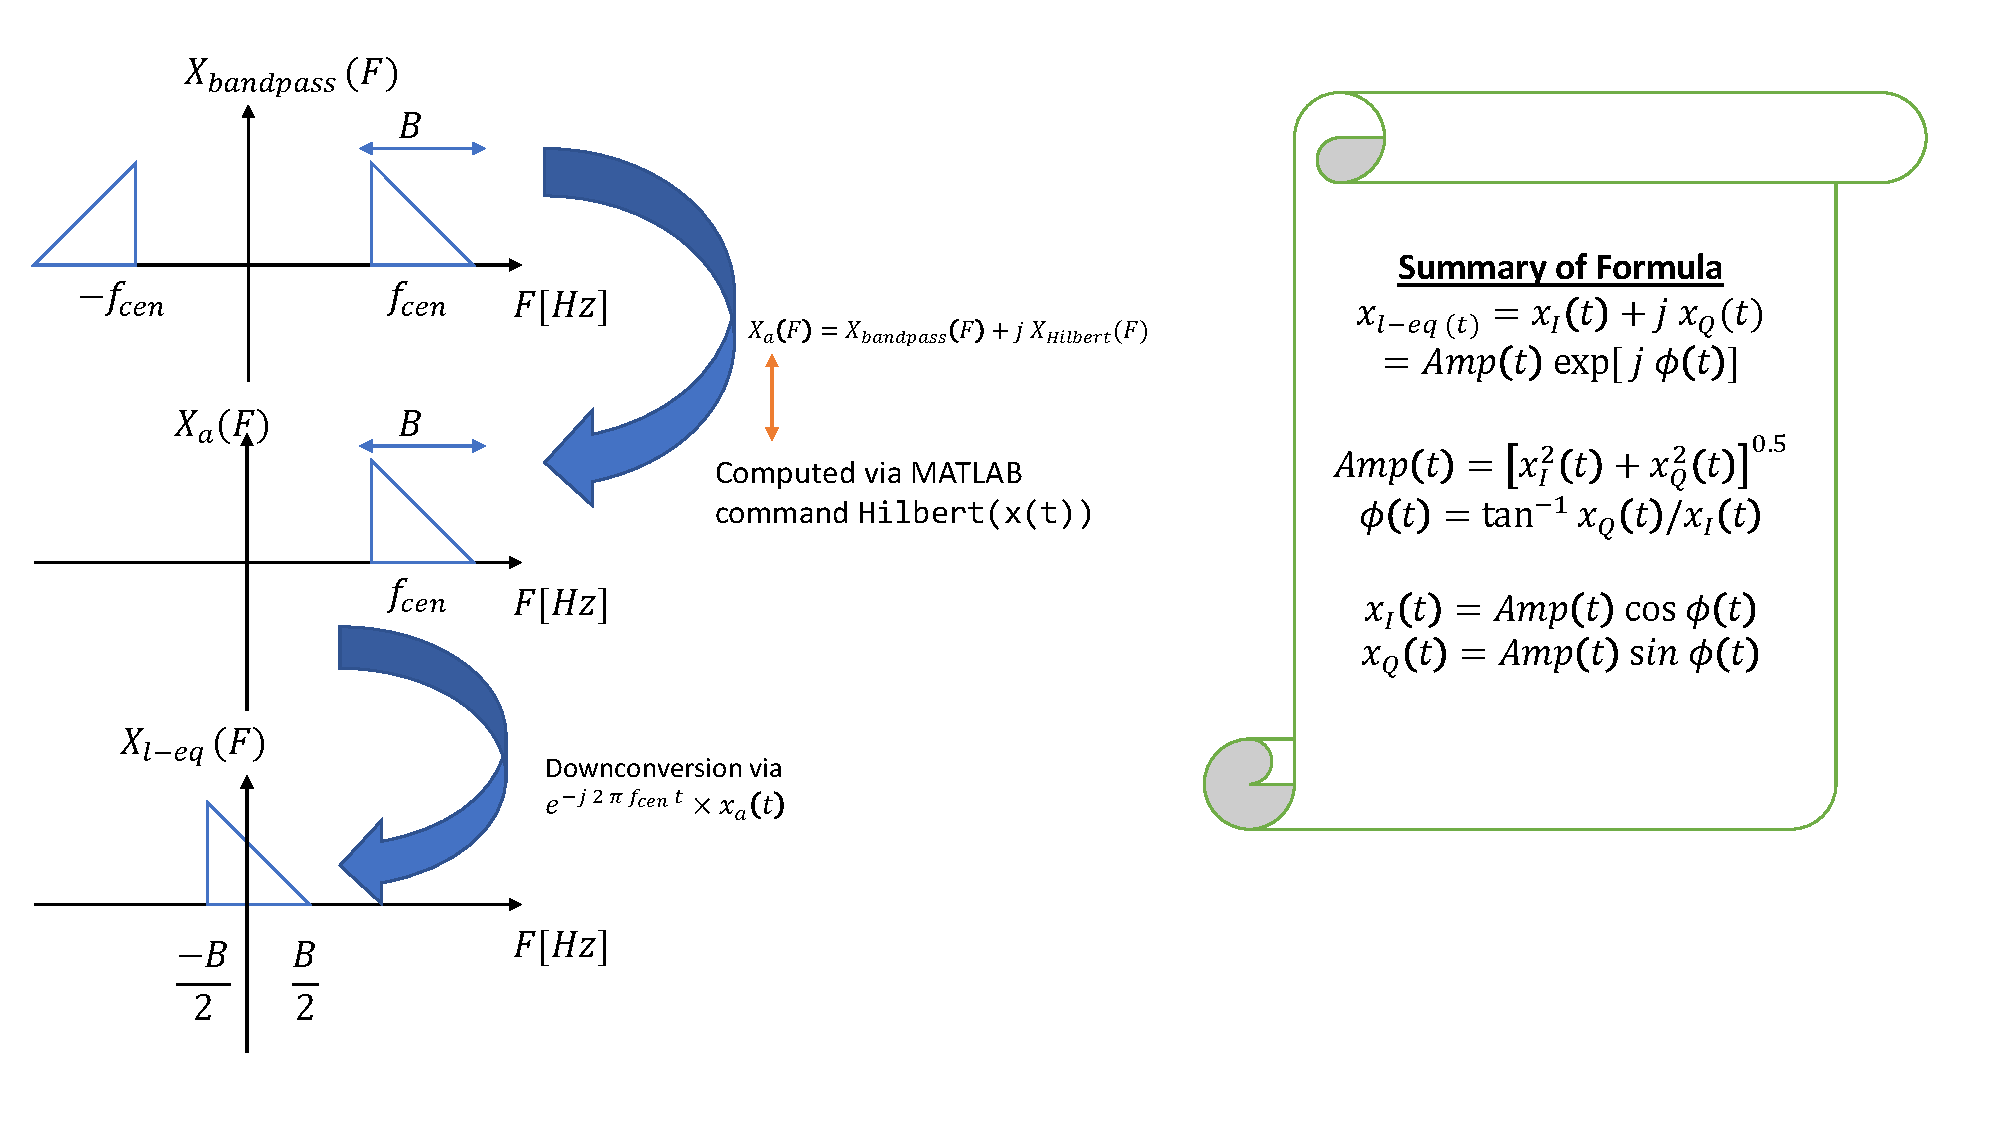
\includegraphics[width = 0.7\textwidth, frame]{Figures/Sampling/summary_IQ}
\caption{Summary for IQ Representation}
\label{fig:Sampling:summary_IQ}
\end{figure}

\subsection{Analog Generation of IQ Signals}

\begin{figure}[h]
\centering
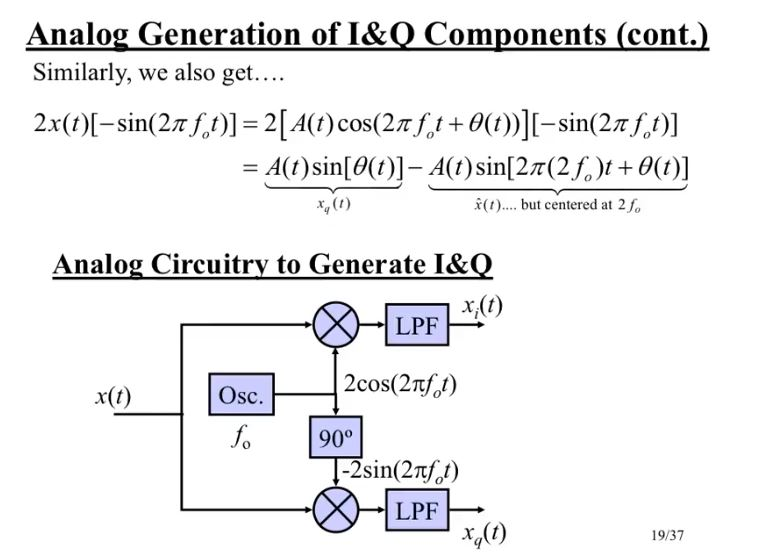
\includegraphics[width = 0.7\textwidth, frame]{Figures/Sampling/qudrature_impelmentation}
\caption{IQ generation and implementation using analog devices}
\label{fig:Sampling:qudrature_impelmentation}
\end{figure}


\newpage
\section{Examples}

\begin{itemize}
    
    \item \todo{FFT leakage}
    
    Ex 5.1 page 175 in \cite{book_SDR_BobStewart}: contains nice explanation about leakage and bins resolution
  
 \end{itemize}
 
 
 \subsection{AM Signals}
 
Let the signal $x(t)$ given by:
 
\begin{equation}
    x(t) \, = \, 
\end{equation} 
 
 \subsection{FM Signals}
 
 
 First we recall the FM signal model:
 
 \begin{equation}
    x_{\text{FM}}(t) \, = \, A_c \, \cos{ \left( \,  2 \pi f_c \, t \, + \, 2 \pi K_{\text{FM}} \, \times \, \displaystyle\int_{- \infty}^t  m(t)\, dt  \,\right)}
\label{Eq:FM:equation_tx}
\end{equation}

In case of FM, $\Phi(t) \, = \, \displaystyle\int_{- \infty}^t  m(t)\, dt$, hence the IQ components are:

\begin{eqnarray}
 I_{\text{FM}}(t) \, &=& \,  A_c \, \cos{ \left(  \, 2 \pi K_{\text{FM}}  \, \displaystyle\int_{- \infty}^t  m(t)\, dt  \,\right)} \\ \\
  Q_{\text{FM}}(t) \, &=& \,  A_c \, \sin{ \left(  \, 2 \pi K_{\text{FM}}  \, \displaystyle\int_{- \infty}^t  m(t)\, dt  \,\right)}
\end{eqnarray}
 
 
 \newpage
\subsection{Design Criteria: Carrier Synchronization and Phase locked Loop}

\underline{Source:} 

\begin{itemize}

\item Begin with a refresher about AM-DSB-SC, section 5 page 182 \cite{book_SDR_BobStewart}

\item Phase Error See section 5.3.3 in \cite{book_SDR_BobStewart} :
    
        \begin{itemize}
            \item In demodulation, the oscillator may not be synchronized with the carrier $\leftrightarrow$ we have some phase $\theta$
            
            \item For a base band message $g(t) \, = \,A \, \cos (2 \pi f_b \, t)$, the demodulation will give: $ \hat{m}(t) \, = \,  \displaystyle\frac{A}{2} \, g(t) \, \cos \, ( \, \theta \, )$
            
            \item for $\theta \, = \, \pm \displaystyle\frac{\pi}{2}$, $\hat{m}(t) \, = \, 0$, that's why we need carrier synchronization and phase locking at the Rx side
            
            
        \end{itemize}
 
\item QAM: a method to transmit 2 data streams on the same carrier, but with a separate offset 

This a more bandwidth efficient scheme.

If we want to compare it to AM-DSB-SC: we need 2 times the bandwidth in AM-DSB-SC for transmission, but in QAM we only need $f_b$.

\begin{itemize}
    \item QAM Tx Side
    
\begin{figure}[h]
\centering
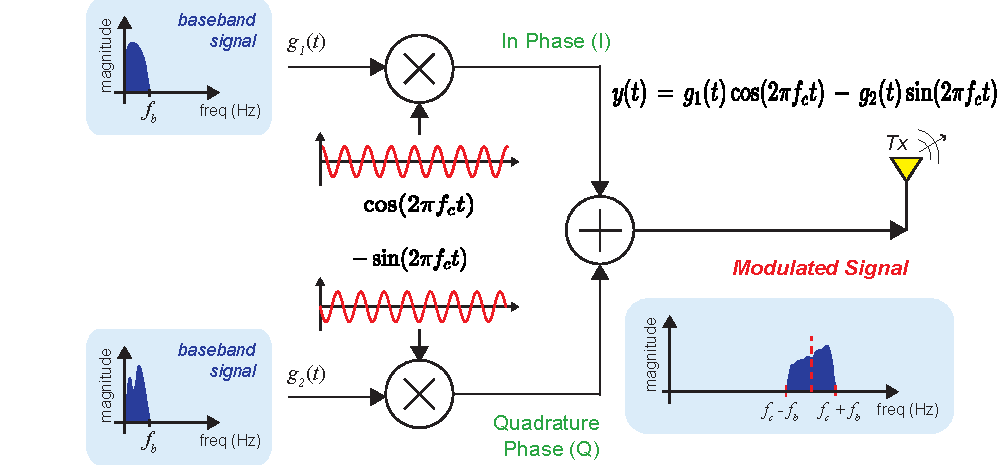
\includegraphics[scale=0.7]{Figures/Complex_Low_Pass/QAM_Tx}
\caption{QAM Tx Side}
\label{fig:Complex_Low_Pass:QAM_Tx}
\end{figure}    
    
    
    \item QAM Rx Side
    
\begin{figure}[h]
\centering
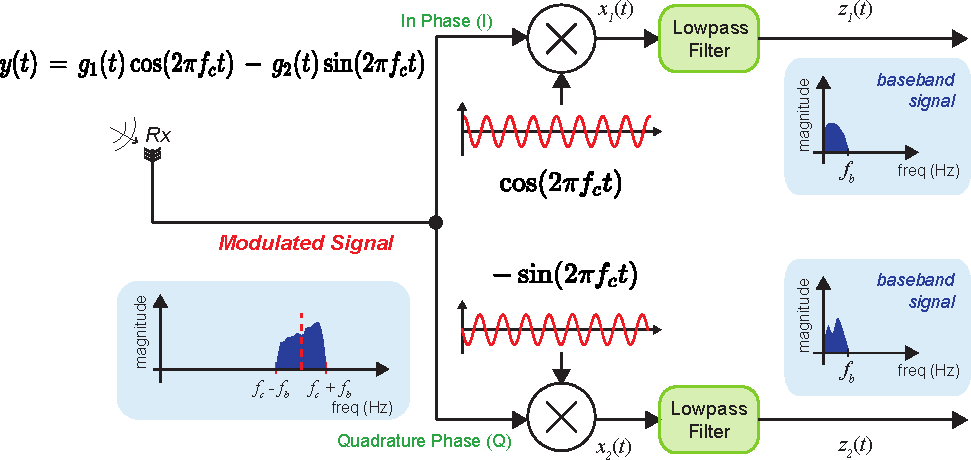
\includegraphics[scale=0.7]{Figures/Complex_Low_Pass/QAM_Rx}
\caption{QAM Rx Side}
\label{fig:Complex_Low_Pass:QAM_Rx}
\end{figure}    
    
    
\end{itemize}

\newpage
\item Using Complex Notation: the key in complex notation is to remember \autoref{Eq:Phasor_Notation}

\begin{equation}
\cos (2 \pi f_c t) \, = \, \text{Re}(e^{j 2 \pi f_c t})    
\label{Eq:Phasor_Notation}
\end{equation}
  
  
\newpage    
In \autoref{fig:Complex_Low_Pass:QAM_Tx_Rx_Complex}, we have the equivalent Tx-Rx QAM scheme using complex notation

\begin{figure}[h]
\centering
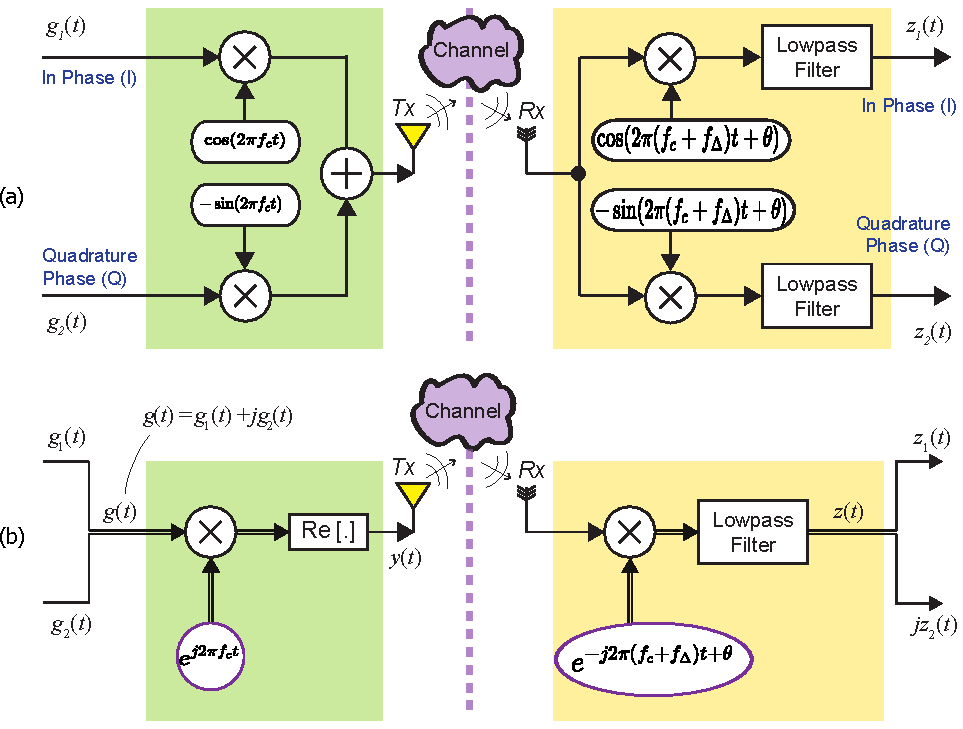
\includegraphics[scale=0.7]{Figures/Complex_Low_Pass/QAM_Tx_Rx_Complex}
\caption{QAM Tx-Rx Using Complex Notation}
\label{fig:Complex_Low_Pass:QAM_Tx_Rx_Complex}
\end{figure}    
    

    
\end{itemize}


%***************************************
%***************************************
%***************************************